\documentclass[12pt]{beamer}
\usepackage{natbib}         % Pour la bibliographie
\usepackage{url}            % Pour citer les adresses web
\usepackage[T1]{fontenc}    % Encodage des accents
\usepackage[utf8]{inputenc} % Lui aussi
\usepackage[frenchb]{babel} % Pour la traduction française
\usepackage{numprint}       % Histoire que les chiffres soient bien

\usepackage{amsmath}        % La base pour les maths
\usepackage{mathrsfs}       % Quelques symboles supplémentaires
\usepackage{amssymb}        % encore des symboles.
\usepackage{amsfonts}       % Des fontes, eg pour \mathbb.

\usepackage{multicol}         % Pour pouvoir séparer l'espace en plusieurs colonnes

%\usepackage[svgnames]{xcolor} % De la couleur
\usepackage{geometry}       % Gérer correctement la taille
\usepackage{array}

\usepackage{tikz, pgfplots}
\usetikzlibrary{positioning} % Add this line to load the positioning library
\usetikzlibrary{fit}

\usepackage{listings}
\usepackage{tcolorbox}

\usepackage{comment}

\usetheme{metropolis}

\title{Le traitement du langage naturel par transformers illustré par un exemple pour la classification de texte}

\author{Cerisara Nathan, MPI}

\begin{document}

\maketitle

%%%%%%%%% PAGE 1 : SOMMAIRE %%%%%%%%%

\begin{frame}{Sommaire}

\begin{itemize}
  \item Architecture Transformer
  	\begin{itemize}
  		\item Vectorisation du texte
  		\item La partie Encodeur de l'architecture
  		\item Les matrices d'Attention
  		\item Le réseau Feed Forward
  	\end{itemize}
  \vspace{7px}
  \item Application personnelle
     \begin{itemize}
      		\item Objectif / Rapport à la ville
      		\item Le modèle BERT
      		\item La structure du réseau de neurone utilisée
      		\item Les données et l'apprentissage
      		\item Les résultats
     \end{itemize}
     \vspace{7px}
     \item Annexes
\end{itemize}

\end{frame}

%%%%%%%%% PAGE 2 : L'architecture Transformer %%%%%%%%%

\begin{frame}{L'architecture Transformer}
Schéma de l'architecture dans le cas de la génération :

\begin{center}

\resizebox{!}{(\textheight * 8 / 11)}{%
\begin{tikzpicture}[
Block/.style =  {rectangle,  rounded corners, draw=black!100, fill =white!0, thick, minimum width = 80px},
Eblock/.style = {rectangle, rounded corners, draw=black!40!green, fill =green!10, thick, minimum height = 30px, minimum width = 100px},
Dblock/.style = {rectangle, rounded corners, draw=black!40!blue, fill =blue!10, thick, minimum height = 30px, minimum width = 100px},
Vect/.style = {circle, draw=purple!80!red, thick, font=\footnotesize, text width=8px, align=left},
Fleche1/.style = {->, thick, shorten <=5px, shorten >=5px},
Fleche2/.style= {->,orange, thick, shorten <=5px, shorten >= 5px},
scale=2
]

%Nodes

%Encoder Blocks
\node[Block] (Tok) {Tokenizer};
\node[Block, align=center] (EPE)  [above=15px of Tok] {Embedding + \\Positional Encoding};
\node[Eblock] (Enc1) [above=15px of EPE] {Encoder $1$};
\node[Eblock] (Enc2) [above=15px of Enc1] {Encoder $2$};
\node (dots1) [above=15px of Enc2] {$\dots$};
\node[Eblock] (EncN) [above=15px of dots1] {Encoder $N_e$};

%Encoder Input
\node (Einp) [below=20px of Tok] {};
\node[font=\footnotesize] (Einp_dots) [right=0px of Einp] {$\dots$};
\node[Vect] (Einp_2) [left=5px of Einp_dots] {$x_2$};
\node[Vect] (Einp_1) [left=5px of Einp_2] {$x_1$};
\node[Vect] (Einp_N) [right=5px of Einp_dots] {$x_N$};
\node (txt_Einp) [left=5px of Einp_1] {Input};

%Encoder Output
\node (Eout) [above=20px of EncN] {};
\node[font=\footnotesize] (Eout_dots) [right=0px of Eout] {$\dots$};
\node[Vect] (Eout_2) [left= 5px of Eout_dots] {$z_2$};
\node[Vect] (Eout_1) [left=5px of Eout_2] {$z_1$};
\node[Vect] (Eout_N) [right=5px of Eout_dots] {$z_N$};
\node (txt_Eout) [left=5px of Eout_1] {Encoder output};

%Decoder Blocks
\node[Dblock] (Dec1) [right=75px of Enc1] {Decoder $1$};
\node[Dblock] (Dec2) [above=15px of Dec1] {Decoder $2$};
\node (dots2) [above=15px of Dec2] {$\dots$};
\node[Dblock] (DecN) [above=15px of dots2] {Decoder $N_d$};
\node[Block, align=center] (Probs) [above=15px of DecN] {Predict the probabilities\\ of the next token};

%Decoder Input
\node (Dinp) [below=20px of Dec1] {};
\node[font=\footnotesize] (Dinp_dots) [right=0px of Dinp] {$\dots$};
\node[Vect] (Dinp_2) [left=5px of Dinp_dots] {$y_2$};
\node[Vect] (Dinp_1) [left=5px of Dinp_2] {$y_1$};
\node[Vect] (Dinp_N) [right=5px of Dinp_dots] {$y_N$};
\node (txt_Dinp) [right=5px of Dinp_N] {Decoder Masked Input};

%Arrows
\draw[Fleche1] (Einp.north) to (Tok.south);
\draw[Fleche1] (Tok.north) to (EPE.south);
\draw[Fleche1] (EPE.north) to (Enc1.south);
\draw[Fleche1] (Enc1.north) to (Enc2.south);
\draw[Fleche1] (Enc2.north) to (dots1.south);
\draw[Fleche1] (dots1.north) to (EncN.south);
\draw[Fleche1] (EncN.north) to (Eout.south);

\draw[Fleche1] (Dinp.north) to (Dec1.south);
\draw[Fleche1] (Dec1.north) to (Dec2.south);
\draw[Fleche1] (Dec2.north) to (dots2.south);
\draw[Fleche1] (dots2.north) to (DecN.south);
\draw[Fleche1] (DecN.north) to (Probs.south);

\draw[Fleche2] (Eout_N.east) .. controls +(right:25px) and +(left:25px) .. (Dec1.west);
\draw[Fleche2] (Eout_N.east) .. controls +(right:25px) and +(left:25px) .. (Dec2.west);
\draw[Fleche2] (Eout_N.east) .. controls +(right:25px) and +(left:25px) .. (DecN.west);
\end{tikzpicture}
}
\end{center}
\end{frame}


%%%%%%%%% PAGE 3 : Tokenisation & Embeddings %%%%%%%%%

\begin{frame}{Vectorisation du texte : Tokenisation du texte}

\textbf{Tokenizer (bert-base-uncased)}

\textbf{Ex1 : }

\ \textit{SENTENCE} : ``Neural Networks are so cool!''\\
\ \textit{TOKENS} : $\begin{array}{ll} [101, 15756, 6125, 2024, 2061, 4658, 999, 102, 0, \dots, 0] \\ \footnotesize \text{[CLS]} \  \text{``neural''} \ \text{``networks''}\  \text{``are''} \ \text{``so''} \ \text{``cool''} \ \text{``!''} \ \text{[SEP]}  \end{array}$

\vspace{15px}

\textbf{Ex2 : }

\ \textit{SENTENCE} : ``Bonjour le monde!''\\
\ \textit{TOKENS} : $\begin{array}{ll} [101, 14753, 23099, 2099, 3393, 23117, 999, 102, 0, \dots, 0] \\ \footnotesize \text{[CLS]} \  \text{``bon''} \ \text{``\#\#jou''}\  \text{``\#\#r''} \ \text{``le''} \ \text{``monde''} \ \text{``!''} \ \text{[SEP]}  \end{array}$

\end{frame}


%%%%%%%%% PAGE 4 : Embeddings + Positional Encoding %%%%%%%%%
\begin{frame}{Vectorisation du texte : Embeddings \& Positional Encoding}


\begin{center}
	\resizebox{(\textwidth * 4 / 5)}{!}{%{(\textheight * 4 / 17)}{
	
	\begin{minipage}{(\textwidth * 21  / 20)}
		
		\setlength{\columnsep}{80pt}
	
		\begin{multicols}{2}[]
		
		\textbf{Positional Encoding}
		
		$$p_k  = (s_0, c_1, \dots, s_{2i}, c_{2i+1}, \dots, s_N)$$
		$$s_{2i} = \sin \left( k \cdot 10000^{- \frac{2i}{d_E}} \right)$$
		$$c_{2i+1} = \cos \left( k \cdot 10000^{- \frac{2i+1}{d_E}} \right)$$
		
		\columnbreak
		
		\textbf{Token Embedding}
		
		$$t_k \longrightarrow \underbrace{(e_{k, 0}, \dots, e_{k, d_E})}_{\text{dimension } d_E}$$
		
		\end{multicols}
	\end{minipage}
	}
\end{center}

\begin{center}
\resizebox{!}{(\textheight * 5 / 18)}{
\begin{tikzpicture}[
Fleche1/.style = {->, thick, shorten <=5px, shorten >=5px}
]

%Blocks

\node (Sentence) {Sentence};
\node (Tokens) [right=15px of Sentence] {Tokens};
\node (TokensT) [below=0px of Tokens] {$T = [t_1, \dots, t_N] \quad$};
\node (EmptySpace) [right=80px of Tokens] {};
\node (TokenEmbedding) [above=15px of EmptySpace] {TokenEmbedding};
\node (EmbeddingE) [above=0px of TokenEmbedding] {$E = [e_1, \dots, e_N]$};
\node (PositionalEncoding) [below=15px of EmptySpace] {Positional Encoding};
\node (PositionalP) [below=0px of PositionalEncoding] {$P = [p_1, \dots, p_N]$};
\node (LayerNorm) [right=80px of EmptySpace] {LayerNormalization $(E + P)$};
\node (Model) [right=15px of LayerNorm] {Model};

  \node [fit=(Sentence) (Model) (EmbeddingE) (PositionalP), draw=red, thick, inner sep=5pt, rounded corners] (box) {};

%Fleches

\draw[Fleche1] (Sentence.east) to (Tokens.west);
\draw[Fleche1] (Tokens.east) to (TokenEmbedding.west);
\draw[Fleche1] (Tokens.east) to (PositionalEncoding.west);
\draw[Fleche1] (TokenEmbedding.east) to (LayerNorm.west);
\draw[Fleche1] (PositionalEncoding.east) to (LayerNorm.west);
\draw[Fleche1] (LayerNorm.east) to (Model.west);

\end{tikzpicture}
}
\end{center}

\end{frame}


%%%%%%%%% PAGE 5 : Vectorisation du texte %%%%%%%%%

\begin{frame}{La partie Encodeur}

Schéma d'un block de la partie Encodeur de l'architecture Transformer :

\begin{center}

\resizebox{!}{(\textheight * 8 / 11)}{%
\begin{tikzpicture}[
EncBlock/.style = {rectangle, rounded corners, draw=green!30, fill=green!5, thick, dashed, minimum width=150px, minimum height=212px},
Block/.style =  {rectangle,  rounded corners, draw=black!100, fill =white!0, thick, minimum width = 80px},
Ablock/.style = {rectangle, rounded corners, draw=black!40!green, fill =green!10, thick, minimum height = 50px, minimum width = 100px},
FFblock/.style = {rectangle, rounded corners, draw=black!40!blue, fill =blue!10, thick, minimum height = 50px, minimum width = 100px},
Vect/.style = {circle, draw=purple!80!red, thick, font=\footnotesize, text width=8px, align=left},
Circ/.style = {circle, draw=black, thick},
Fleche1/.style = {->, thick, shorten <=5px, shorten >= 5px},
]

%Encoder Input
\node (Einp) {};
\node[font=\footnotesize] (Einp_dots) [right=0px of Einp] {$\dots$};
\node[Vect] (Einp_2) [left=5px of Einp_dots] {$x_2$};
\node[Vect] (Einp_1) [left=5px of Einp_2] {$x_1$};
\node[Vect] (Einp_N) [right=5px of Einp_dots] {$x_N$};
\node (txt_Einp) [left=5px of Einp_1] {Input};

%Global Encoder Block
\node[EncBlock] (Enc) [above=10px of Einp] {};
\node (Txt_Encoder) [left=8px of Enc] {Encoder Block};

% MultiHead Self-Attention Block
\node[Ablock] (Att) [above=15px of Einp] {MultiHead Self-Attention};
\node[Block] (AN1) [above=15px of Att] {Add \& Normalize};

%Attention output
\node (Aout) [above=15px of AN1] {};
\node[font=\footnotesize] (Aout_dots) [right=0px of Aout] {$\dots$};
\node[Vect] (Aout_2) [left=5px of Aout_dots] {$x_2$};
\node[Vect] (Aout_1) [left=5px of Aout_2] {$x_1$};
\node[Vect] (Aout_N) [right=5px of Aout_dots] {$x_N$};

%FF block
\node[FFblock] (FF) [above=15px of Aout] {Feed Forward Layer};
\node[Block] (AN2) [above=15px of FF] {Add \& Normalize};

%Encoder Output
\node (Eout) [above=15px of AN2] {};
\node[font=\footnotesize] (Eout_dots) [right=0px of Eout] {$\dots$};
\node[Vect] (Eout_2) [left=5px of Eout_dots] {$x_2$};
\node[Vect] (Eout_1) [left=5px of Eout_2] {$x_1$};
\node[Vect] (Eout_N) [right=5px of Eout_dots] {$x_N$};
\node (txt_Eout) [left=5px of Eout_1] {Output};

%Arrows
\draw[Fleche1] (Einp.north) to (Att.south);
\draw[Fleche1] (Att.north) to (AN1.south);
\draw[Fleche1] (AN1.north) to (Aout.south);
\draw[Fleche1] (Aout.north) to (FF.south);
\draw[Fleche1] (FF.north) to (AN2.south);
\draw[Fleche1] (AN2.north) to (Eout.south);

\draw[Fleche1] (Einp_N.east) .. controls +(right:45px) and +(right:45px) ..  node[Circ,scale=0.7, fill=white]{$+$}  (AN1.east);
\draw[Fleche1] (Aout_N.east) .. controls +(right:45px) and +(right:45px) .. node[Circ,scale=0.7, fill=white] {$+$} (AN2.east);
\end{tikzpicture}
}
\end{center}
\end{frame}

%%%%%%%%% PAGE 6 : Matrices d'attention %%%%%%%%%

\begin{frame}{Matrice d'attention}


\begin{center}

\resizebox{(\textwidth * 11 / 11)}{!}{%
\begin{tikzpicture}[
EncBlock/.style = {rectangle, rounded corners, draw=green!30, fill=green!5, thick, dashed, minimum width=150px, minimum height=212px},
Block/.style =  {rectangle,  rounded corners, draw=black!100, fill =white!0, thick, minimum width = 80px},
Ablock/.style = {rectangle, rounded corners, draw=black!40!green, fill =green!10, thick, minimum height = 50px, minimum width = 100px},
FFblock/.style = {rectangle, rounded corners, draw=black!40!blue, fill =blue!10, thick, minimum height = 50px, minimum width = 100px},
Vect/.style = {circle, draw=purple!80!red, thick, font=\footnotesize, text width=8px, align=left},
Circ/.style = {circle, draw=black, thick},
Fleche1/.style = {->, thick, shorten <=5px, shorten >= 5px},
]

\node (X) {$X$};
\node (dimX) [below=0px of X] {$(N, d_E)$};
\node[fit=(X) (dimX), draw=black, thick, rounded corners, inner sep=5px] (boxX) {};

\node (K) [right=100px of X] {$K$};
\node (dimK) [below=0px of K] {$(N, d_k)$};
\node[fit=(K) (dimK), draw=black, fill=orange!20!, thick, rounded corners, inner sep=5px] (boxK) {};
\node (K) [right=100px of X] {$K$};
\node (dimK) [below=0px of K] {$(N, d_k)$};

\node (Empty1) [above=25px of K] {};

\node (Q) [above=25px of Empty1] {$Q$};
\node (dimQ) [below=0px of Q] {$(N, d_k)$};
\node[fit=(Q) (dimQ), draw=black, fill=red!20!, thick, rounded corners, inner sep=5px] (boxQ) {};
\node (Q) [above=25px of Empty1] {$Q$};
\node (dimQ) [below=0px of Q] {$(N, d_k)$};

\node (Empty2) [below=25px of K] {};

\node (V) [below=25px of Empty2] {$V$};
\node (dimV) [below=0px of V] {$(N, d_k)$};
\node[fit=(V) (dimV), draw=black, fill=blue!20!, thick, rounded corners, inner sep=5px] (boxV) {};
\node (V) [below=25px of Empty2] {$V$};
\node (dimV) [below=0px of V] {$(N, d_k)$};

\node (softmax) [right=75px of Empty1] {$\displaystyle \text{softmax} \left ( \frac{QK^\top}{\sqrt{d_k}} \right )$};
\node[fit=(softmax), draw=black, fill=yellow!20!, thick, rounded corners, inner sep=10px] (boxS) {};
\node (softmax) [right=75px of Empty1] {$\displaystyle \text{softmax} \left ( \frac{QK^\top}{\sqrt{d_k}} \right )$};

\node (Empty3) [below=10px of softmax] {};

\node (Y) [below right=5px and 75px of boxS] {$Y$};
\node (dimY) [below=0px of Y] {$(N, d_E)$};
\node[fit=(Y) (dimY), draw=black, thick, rounded corners, inner sep=5px] (boxY) {};

\node (form) [below right=85px and -65px of Empty3] {\large$\text{Attention}(Q, K, V) = \text{softmax} \left ( \frac{QK^\top}{\sqrt{d_k}} \right )V$};

  \node [fit=(form), draw=red, thick, inner sep=5pt, rounded corners] (box) {};


\draw[Fleche1] (boxX.east) to node[left] {$\cdot W_Q$} (boxQ.west);
\draw[Fleche1] (boxX.east) to node[above] {$\cdot W_K$} (boxK.west);
\draw[Fleche1] (boxX.east) to node[left] {$\cdot W_V$} (boxV.west);
\draw[Fleche1] (boxQ.east) to (boxS.west);
\draw[Fleche1] (boxK.east) to (boxS.west);
\draw[Fleche1] (boxS.east) to (boxY.west);
\draw[Fleche1] (boxV.east) to (boxY.west);

\end{tikzpicture}
}
\end{center}

\end{frame}

%%%%%%%%% PAGE 7 : Le réseau Feed Forward %%%%%%%%%

\begin{frame}{Le réseau Feed Forward}


\setlength{\columnsep}{50pt}
\begin{multicols*}{2}[]

\begin{center}
\resizebox{(\textwidth * 6/ 11)}{!}{%
\begin{tikzpicture}[
Lin/.style = {rectangle, rounded corners, draw=red!30!yellow!50, fill =yellow!10, dashed, thick, minimum height = 15px, minimum width = 150px},
Vect/.style = {circle, draw=purple!150!red, thick, font=\footnotesize, text width=8px, align=left},
Vect2/.style = {circle, draw=purple!150!red, thick, font=\footnotesize, text width=8px, align=left},
Circ/.style = {circle, draw=black, thick},
Trait/.style = {-, shorten <=1px, shorten >= 1px},
]


%FF Input
\node (FFinp) {};
\node[font=\footnotesize] (FFinp_dots) [right=0px of FFinp] {$\dots$};
\node[Vect] (FFinp_2) [left=10px of FFinp_dots] {$x_2$};
\node[Vect] (FFinp_1) [left=10px of FFinp_2] {$x_1$};
\node[Vect] (FFinp_N) [right=10px of FFinp_dots] {$x_N$};
\node (txt_FFinp) [left=10px of FFinp_1] {Input $X$};

%Linear1
\node[Lin] (Lin1) [above=15px of FFinp] {};
\node (Txt_lin1) [left=5px of Lin1] {Linear Layer 1};

%Hidden Layer
\node (Hl) [above= 15px of Lin1] {};
\node[font=\footnotesize] (Hl_dots) [above= 45px of FFinp] {$\dots$};
\node[Vect] (Hl_2) [left=10px of Hl_dots] {$h_2$};
\node[Vect] (Hl_1) [left=10px of Hl_2] {$h_1$};
\node[Vect2, minimum width=28px] (Hl_D1) [right=10px of Hl_dots] {$\!\!\!\! h_{D-1}$};
\node[Vect] (Hl_D) [right=10px of Hl_D1] {$h_D$};
\node (txt_Hl) [left=10px of Hl_1] {Hidden State $H$};

%Linear2
\node[Lin] (Lin2) [above=15px of Hl_dots] {};
\node (Txt_lin2) [left=5px of Lin2] {Linear Layer 2};

%FF Output
\node (FFout)  [above=15px of Lin2] {};
\node[font=\footnotesize] (FFout_dots) [right=0px of FFout] {$\dots$};
\node[Vect] (FFout_2) [left=10px of FFout_dots] {$y_2$};
\node[Vect] (FFout_1) [left=10px of FFout_2] {$y_1$};
\node[Vect] (FFout_N) [right=10px of FFout_dots] {$y_N$};
\node (txt_FFout) [left=10px of FFout_1] {Output $Y$};

%Nodes Connections
\draw[Trait] (FFinp_1.north) to (Hl_D.south);
\draw[Trait] (FFinp_1.north) to (Hl_D1.south);
\draw[Trait] (FFinp_1.north) to (Hl_2.south);
\draw[Trait] (FFinp_1.north) to (Hl_1.south);

\draw[Trait] (FFinp_2.north) to (Hl_D.south);
\draw[Trait] (FFinp_2.north) to (Hl_D1.south);
\draw[Trait] (FFinp_2.north) to (Hl_2.south);
\draw[Trait] (FFinp_2.north) to (Hl_1.south);

\draw[Trait] (FFinp_N.north) to (Hl_D.south);
\draw[Trait] (FFinp_N.north) to (Hl_D1.south);
\draw[Trait] (FFinp_N.north) to (Hl_2.south);
\draw[Trait] (FFinp_N.north) to (Hl_1.south);

\draw[Trait] (FFout_1.south) to (Hl_D.north);
\draw[Trait] (FFout_1.south) to (Hl_D1.north);
\draw[Trait] (FFout_1.south) to (Hl_2.north);
\draw[Trait] (FFout_1.south) to (Hl_1.north);

\draw[Trait] (FFout_2.south) to (Hl_D.north);
\draw[Trait] (FFout_2.south) to (Hl_D1.north);
\draw[Trait] (FFout_2.south) to (Hl_2.north);
\draw[Trait] (FFout_2.south) to (Hl_1.north);

\draw[Trait] (FFout_N.south) to (Hl_D.north);
\draw[Trait] (FFout_N.south) to (Hl_D1.north);
\draw[Trait] (FFout_N.south) to (Hl_2.north);
\draw[Trait] (FFout_N.south) to (Hl_1.north);
\end{tikzpicture}
}
\end{center}

\columnbreak

Couche linéaire : $X \mapsto X\cdot W^\top + B$

\end{multicols*}

\end{frame}


%%%%%%%%% PAGE 8 : Le réseau Feed Forward %%%%%%%%%

\begin{frame}{Application Personnelle: Objectifs \& Rapport à la ville}


\begin{itemize}
	\item \textbf{Objectif :}
	\begin{itemize}
		\item Classification de texte
		\item Sentiment : Négatif $\longleftrightarrow$ Positif
	\end{itemize}
	\item \textbf{Rapport à la ville :}
	\begin{itemize}
		\item Analyser les sentiments des habitants sur différents sujets
	\end{itemize}
\end{itemize}


\end{frame}


%%%%%%%%% PAGE 9 : Le modèle BERT %%%%%%%%%

\begin{frame}{Le modèle BERT}

\begin{itemize}
	\item Architecture Transformer
	\item Plusieurs tailles de BERT (base, large, ...)
	\item BERT base : $12 \times$ blocks encoder $\to 112$M paramètres 
	\item BooksCorpus (800M words) and English Wikipedia (2,500M words)
	\item Publié vers fin 2018 par des chercheurs de Google
\end{itemize}

\end{frame}


%%%%%%%%% PAGE 10 : La structure du réseau de neurone utilisée %%%%%%%%%

\begin{frame}{La structure du réseau de neurone utilisée}


\begin{center}

\resizebox{(\textwidth)}{!}{%
\begin{tikzpicture}[
EncBlock/.style = {rectangle, rounded corners, draw=green!30, fill=green!5, thick, dashed, minimum width=150px, minimum height=212px},
Block/.style =  {rectangle,  rounded corners, draw=black!100, fill =white!0, thick, minimum width = 80px, align=center},
Bblock/.style = {rectangle, rounded corners, draw=black!40!green, fill =green!10, thick, minimum height = 50px, minimum width = 100px, align=center},
FFblock/.style = {rectangle, rounded corners, draw=black!40!blue, fill =blue!10, thick, minimum height = 50px, minimum width = 100px, align=center},
Vect/.style = {circle, draw=purple!80!red, thick, font=\footnotesize, text width=8px, align=left},
Circ/.style = {circle, draw=black, thick},
Fleche1/.style = {->, thick, shorten <=5px, shorten >= 5px},
]

%Blocks
\node (Inp) {``Input''};
\node[Block] (BT) [right=25px of Inp] {BERT\\Tokenizer};
\node[Bblock] (BE) [right=25px of BT] {BERT\\Encoder};
\node[FFblock] (FFC) [right=25px of BE] {Feed Forward\\Classifier};
\node[Vect] (Out) [right=25px of FFC] {$c$};

%Arrows
\draw[Fleche1] (Inp.east) to (BT.west);
\draw[Fleche1] (BT.east) to (BE.west);
\draw[Fleche1] (BE.east) to (FFC.west);
\draw[Fleche1] (FFC.east) to (Out.west);

\end{tikzpicture}
}
\end{center}



\end{frame}


%%%%%%%%% PAGE 11 : Les données et l'apprentissage %%%%%%%%%

\begin{frame}{Les données et l'apprentissage}

\begin{itemize}
	\item \textbf{Données : } Standford Sentiment Dataset
	\item Train : 8544, Test : 2210
	\item \textbf{Temps d'entraînement : } $\approx$ 15min
	\item \textbf{Algorithme d'apprentissage : } Adam optimizer (extension de la descente de gradient stochastique)
	\item \textbf{Fonction de Loss : } MinSquaredError
\end{itemize}

\end{frame}



%%%%%%%%% PAGE 12 : Les résultats %%%%%%%%%

\begin{frame}{Les résultats}

\begin{center}
\resizebox{(\textwidth * 11 / 11)}{!}{
\begin{tikzpicture}

\node (LossTest) {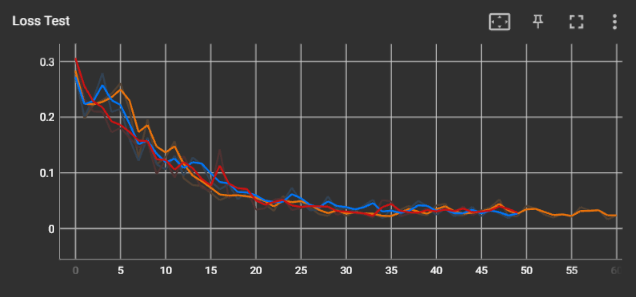
\includegraphics{loss_test.png}};
\node (LossTrain) [right= of LossTest] {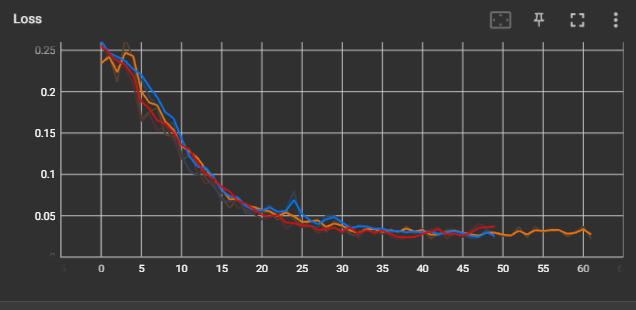
\includegraphics{loss_train.png}};

\end{tikzpicture}
}
\end{center}

\end{frame}



%%%%%%%%% PAGE 13 : Annexes %%%%%%%%%

\begin{frame}{Annexes}


\begin{center}
	\resizebox{(\textwidth * 9 / 10)}{!}{%{(\textheight * 4 / 17)}{
	
	\begin{minipage}{(\textwidth * 21  / 20)}
		
\setlength{\columnsep}{1pt}
\begin{multicols*}{2}[]

\textbf{Ce que l'on a vu :}

\begin{itemize}
	\item Architecture Transformer
	\begin{itemize}
		\item Le block d'encodeur
		\item Les matrices d'attention
		\item Les réseaux Feed Forward
	\end{itemize}
	\item Application Personnelle
\end{itemize}

\columnbreak

\textbf{Annexes / Ouvertures :}

\begin{itemize}
	\item Détails du code python
	\item Adam optimizer
	\item La fonction de loss
	\item La Normalisation par couche (LayerNorm)
	\item La partie décodeur
	\item Comparaison avec le modèle GPT
	\item Le théorème d'approximation universel
	\item Bibliographie
\end{itemize}

\end{multicols*}
	\end{minipage}
	}
\end{center}



\end{frame}



%%%%%%%%% PAGE 14 : Annexe - Python %%%%%%%%%

\begin{frame}[fragile]{Annexes: Code python}
\footnotesize
\begin{tcolorbox}[colback=white,boxsep=2mm,arc=1pt,
    auto outer arc,left=1mm,right=1mm,top=1mm,bottom=1mm,boxrule=0.5pt,width=\textwidth]
\begin{lstlisting}[language=python]
import torch.nn as nn

class Net(nn.Module):  
    def __init__(self, dim_in, dim_out):
        super().__init__()
        #
        self.layer = nn.Linear(dim_in, dim_out)

    def forward(self, x):
        return self.layer(x)
\end{lstlisting}
\end{tcolorbox}
\normalsize
\end{frame}



%%%%%%%%% PAGE 15 : Annexe - L'algorithme de backpropagation %%%%%%%%%

\begin{frame}{Annexes: Adam Optimizer}



\end{frame}




%%%%%%%%% PAGE 16 : Annexe - Fonction de loss %%%%%%%%%

\begin{frame}{Annexes: Fonction de loss}



\end{frame}




%%%%%%%%% PAGE 17 : Annexe - LayerNormalization %%%%%%%%%

\begin{frame}{Annexes: LayerNormalization}



\end{frame}




%%%%%%%%% PAGE 18 : Annexe - Partie décodeur de l'architecture transformer %%%%%%%%%

\begin{frame}{Annexes: Partie décodeur de l'architecture transformer}



\end{frame}



%%%%%%%%% PAGE 19 : Annexe - Comparaison avec le modème GPT %%%%%%%%%

\begin{frame}{Annexes: Comparaison avec le modèle GPT}



\end{frame}





%%%%%%%%% PAGE 20 : Annexe - Le théorème d'approximation universel %%%%%%%%%

\begin{frame}{Annexes: Le théorème d'approximation universel}

\textbf{Enoncé :}
Les transformateurs sont des approximateurs universels des fonctions continues de séquence à séquence sur un domaine compact.

\textbf{Preuve :}



\end{frame}




%%%%%%%%% PAGE 21 : Annexe - Bibliographie %%%%%%%%%

\begin{frame}{Annexes: Bibliographie}

\begin{itemize}
	\item Les différents papiers 
	\item ``ARE TRANSFORMERS UNIVERSAL APPROXIMATORS
OF SEQUENCE-TO-SEQUENCE FUNCTIONS?'', Google Research 2020
\end{itemize}

\end{frame}







\end{document}